\chapter{Implementation}
\label{sec:implementation}
\minitoc
\vspace*{1cm}

This chapter is dedicated to the technical aspects involved while exploring some of the key characteristics that constitute \pname{}. In depth, we look at the coding standards used when developing this fuzzing tool, exploiting Asynchronous I/O to achieve concurrency in Python, the parsing procedure of a response and a user-friendly interface displaying statistics. Additionally, useful information is given about operating \pname{}.

% NEW SECTION
\section{Coding Standards}
Guido van Rossum(creator of the Python programming language) said; "Code is read much more often than it is written". For this reason, throughout this thesis, our main aim was to write clean, readable and eye-pleasing code by following best practice that the best professional tools adhere to. In so doing, we applied the latest conventions, as recommended by the Python community to enforce maintainability, clarity, consistency, and generally, a foundation for good programming habits and practices. 

More specifically, our fuzzing tool is fully written in Python 3.8 using the PEP 8 ~\cite{python_pep8} coding style standard and, regarding documentation, the PEP 257 ~\cite{python_pep257} and Sphinx ~\cite{sphinx} docstring conventions were adopted for it to be clear and easy to read for programmers. Pylint ~\cite{pylint_module} was also used to check for errors in Python code and to implement the aforementioned coding standards and search for code smells.

To enhance good practise, unit tests were created through which individual modules of the tool's source code were put under different tests to determine a particular unit's correctness and whether it is fit for purpose. More precisely, parts of the application's code are validated by using test cases that stress-test the tool and ascertain the quality of the code by checking it against the expected response. For this part, popular python test frameworks were used like pytest ~\cite{pytest_module}, unittest ~\cite{unittest_module} and mock ~\cite{mock}. In the appendix, an example of unit testing for the Parser module can be found.

% NEW SECTION
\section{Asynchronous I/O}
\pname{} utilises concurrent programming (see Section ~\ref{sec:background}) with the help of the asyncio ~\cite{asyncio} Python module. In our case, asyncio has made it possible to send, continuously, HTTP requests to the target website while at the same time statistics on the fuzzing session are printed on the user's screen and a respective log file is updated. With assistance from the aforementioned module, some of the potential speed-bumps that we might otherwise encounter; such as logging request information to a file or waiting idly for a response for each request, were overcome, since any I/O operation caused by a blocking function does not forbid others from running. Conversely, it allows other functionalities to run from the time that it starts until the time that it returns. 

Multiple asynchronous tasks (also known as routines) cooperate to let each other take turns running using the {\tt await} keyword, to yield optimal performance. This keyword enables tasks to pause while they wait for their results and let other tasks run in the meantime. This process is called cooperative multitasking and although it involves doing extra work up front, the benefit is that you always know when your task will be swapped out, thus optimising to yield better performance.

To summarise, the concept of asyncio is that a single-threaded Python object, called the event loop, controls how and when each task is run. Each task can either be in ready state, which means that the task has work to do and is ready to be run while the waiting state means the task is waiting for some external thing to finish, such as a network operation. The event loop is aware of each task and knows what state it is in and maintains two lists of tasks, one for each of these states. 

It selects one of the ready tasks and then returns it back to running. That task is in complete control until it cooperatively hands the control back to the event loop, which in turn places that task into either the ready or waiting list and chooses another task to run. It is important to note, that the tasks never give up control without intentionally doing so using {\tt await}, hence, they are never interrupted in the middle of an operation. A detailed depiction of the asynchronous process executed by asyncio can be viewed in Figure ~\ref{fig:asyncio_image_source}.

\begin{figure}[ht]
 \centering
 \captionsetup{justification=centering}
 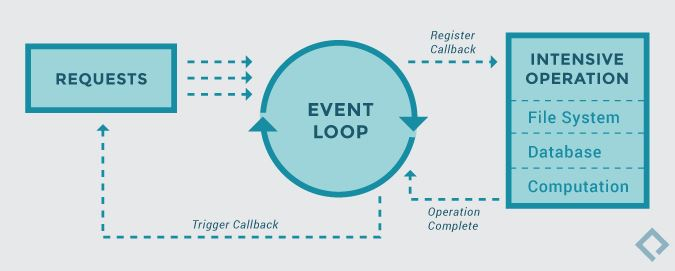
\includegraphics[width=\linewidth]{figures/asyncio_process.jpg}
 \caption[AsyncIO mechanism]
 {AsyncIO mechanism; it provides a high-performance asynchronous frameworks for making our fuzzing requests ~\cite{asyncio_image_source}}
 \label{fig:asyncio_image_source}
\end{figure}

Communication with the target's website is achieved with a rapidly fast asynchronous http client/server framework named aiohttp ~\cite{aiohttp}. The aiohttp module creates a reusable Session object per web application through which all requests are performed. Since our fuzzer works with one web application per execution, a single session is created, shared across all tasks, and reused for the entire execution of the program. The re-usability of the session is feasible because all tasks are running on the same thread. Pairing aiohttp with asyncio evidently speeds things up.

It is important to note here that not all available Python modules are compatible with asyncio. For our requests, we could not use the default and recommended Python requests package, since it is built on top of {\tt urllib3 }, which in turn uses Python's http and socket modules. Socket operations are blocking and not  {\tt awaitable } which signals that Python will not like the {\tt await } statement. However, more modules are becoming compatible with asyncio ~\cite{aiohttp}.

\section{Parser}
The fuzzer's parsing module is responsible for extracting vital information during the fuzzing process from each response received, after, of course, the respective request is made. Each response contains the HTML document which is then parsed using the {\tt  Beautiful Soup } ~\cite{beautiful_soup} module to extract the form and anchor elements from it. These elements are useful as they can provide us with new URLs which translate into potentially new code paths and bugs to further explore and locate. 

When new URLs are found, they are added to the crawler's pending request list, if they are interesting (see Section ~\ref{sec:architecture}) they will also be fuzzed in the future. At this stage the HTML document is also checked for XSS vulnerabilities. The metadata that we stored for each request, can tell us which XSS payloads were injected into it and led to this vulnerability. If they happen to reside in the HTML document, which signal an RXSS vulnerability, a warning is triggered, incrementing the total number of XSS found and logging the related information. The document is also checked for Stored XSS vulnerabilities by scanning the document for all the XSS payloads that were injected in all the requests. A high-level pseudo-code for the parsing process can be seen at Algorithm ~\ref{alg:parser_pseudocode}. 

As the pseudo-code shows clearly, parsing relies heavily on the urllib.parse~\cite{urllib_parse} Python module. This module, more precisely the urlparse method, is used for breaking the Uniform Resource Locator (URL) string up into components; such as the addressing scheme, network location, path \etc An object is returned that contains 6-item tuple with all the URL sub-fields. The reverse can also be achieved through the urlunparse method; a URL object can be converted into string.

\begin{algorithm}
 
 \caption{Parsing new HTML documents method pseudocode.}
 \label{alg:parser_pseudocode}
 
 \begin{algorithmic}
	\STATE lookForXSS(HTML) \COMMENT{Increments global XSS counter if one is found.} 
	\STATE $links \leftarrow set()$ 
	\FOR{every form found in the HTML document}
		 \IF{form does \NOT contain an action field}
 			\STATE $urlObject \leftarrow urllib.parse(callingNodeUrl)$
		 \ELSE 
 			\STATE $urlObject \leftarrow urllib.parse(relativeToAbsolute(form.action))$
		 \ENDIF
		\STATE $parameters \leftarrow parseQueryString(urlObject.query)$ 
		\STATE $urlString \leftarrow urllib.unparse(urlObject)$ 
		\STATE $inputs \leftarrow dictionary()$ 
		\FOR{every < input > element found in form}
			\STATE $value \leftarrow input.get(value)$			 
	 		\STATE $name \leftarrow input.get(name)$	
	 		\STATE $inputs[name] \leftarrow append(value)$	 
		\ENDFOR
		\STATE $method \leftarrow form.get(method)$	
		\STATE $Node \leftarrow createNode(parameters, urlString, inputs, method)$	
		\STATE $links \leftarrow add(Node)$
		\FOR{every < a > element found in form}
			\STATE $anchor \leftarrow a.get(href)$			 
		\ENDFOR
		\STATE $Node \leftarrow createNode(parameters, urlString, inputs, method)$	
		\STATE $links \leftarrow add(Node)$
	\ENDFOR
	\RETURN links
 \end{algorithmic}
\end{algorithm}

\section{Curses Interface}
A Textual User Interface (TUI) for \pname{} has been created using the curses module which contains information and essential statistics, gathered while our grey-box fuzzer is running. The curses library supplies a terminal-independent screen-painting and keyboard-handling facility for text-based terminals~\cite{curses}, such as the Linux console. The text editor \textit{nano} is a good example of a curses application. 

Unfortunately, this functionality is not available for Windows, as the Windows version of Python does not include the curses module. So by running our fuzzing tool on a Windows-based machine, regardless of the Command Line Interface (CLI) you opt to use, it will result in a crash. 

There are of course ways to run \pname{} without this interface which will be explained in the next sub-section. Although many may think this is obsolete technology, it can prove to be  valuable for Unix-based operating systems that do not provide any graphical support. The Python module, which is the one we utilised, is a fairly simple wrapper over the \textit{C} functions provided by the first and original curses. A snapshot of the interface provided by webFuzz can be seen in Figure ~\ref{fig:curses_interface}. As illustrated, the statistics are divided into three categories; namely the process statistics, the overall progress and the examining node details.
As the fuzzing tool expands, more valuable information is expected to be included on the interface.

\begin{figure}[ht]
 \centering
 \captionsetup{justification=centering}
 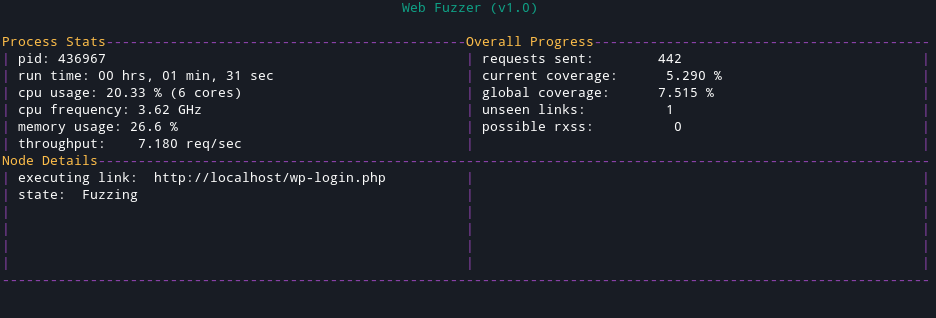
\includegraphics[width=\linewidth]{figures/curses.png}
 \caption[Interface of webFuzz]
 {Interface of webFuzz. The interface is implemented using the Curses module}
 \label{fig:curses_interface}
\end{figure}

\section{Running webFuzz}
Running \pname{} is straightforward. All necessary modules accompanied with their exact version needed to be installed for \pname{} to work smoothly. These are listed in a "requirements" text file. Other executing and installing dependency instructions can be found at the README.md file in the tool's repository.

A help menu that shows all available arguments in which \pname{} can run in, are shown in Figure ~\ref{fig:argparser_menu}. As you can see, arguments are separated in three categories; namely \emph{Optional}, \emph{Required} and \emph{Positional}. Optional arguments are extra functionalities that you do not have to include when running the tool, whereas Required and Positiona are the arguments that must be included. For the creation of the usage menu and parsing the arguments, the argparse~\cite{argparse} Python module was used.

Also, throughout the execution, logging is used as a means of tracking events that happen when the fuzzer runs. Logging is a module in the Python standard library that provides a richly-formatted log.

\begin{figure}[ht]
 \centering
 \captionsetup{justification=centering}
 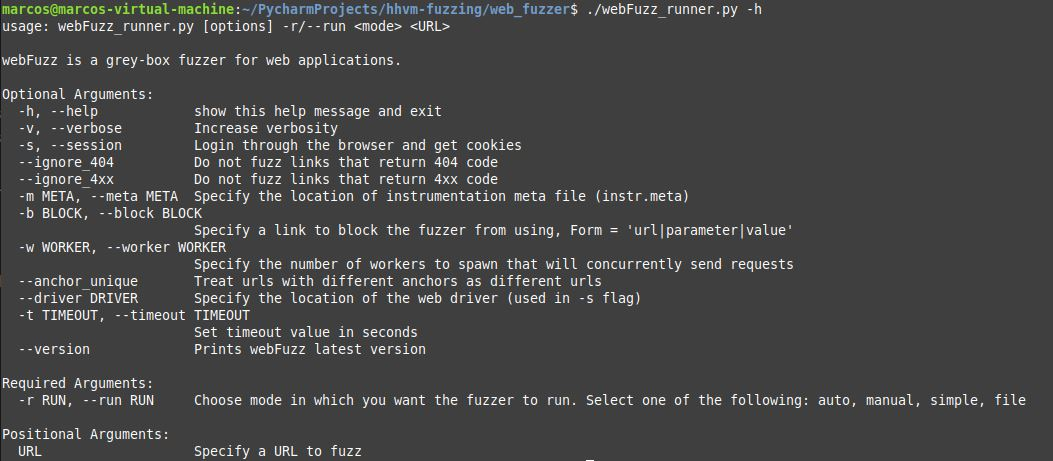
\includegraphics[width=\linewidth]{figures/argparser_menu.jpg}
 \caption[\pname{} usage menu]{\pname{} usage menu includes all available arguments which we can use to run it with}
 \label{fig:argparser_menu}
\end{figure}

\section{Interactive and Black-Box Functionalities}
Our fuzzing tool provides manual functionality also. This functionality allows the user to engage through an interactive session with our fuzzer. After the user provides the target to be fuzzed, a connection its establish and the session begins. Before a request is made, forms are extracted from the target and all input fields are presented to the user. Then, the user chooses from a menu of option which fields to fuzz and how. More specifically, options consist of filling the fields with manually inserted data, with XSS payloads from the corpus previously seen at Table \ref{xss_payload_tables} or choosing to mutate data using a basic mutating function. Mutating functions for a given input provided include deleting random characters, inserting characters ate random places and flipping random characters. The user must insert manually any different link desired to be fuzzed, as no crawling process is provided. At Listing ~\ref{lst:interactive_mode}, we can see a code snippet of the interactive mode. 

\begin{lstlisting}[showstringspaces=false, frame=single, language=Python, caption={Options menu and their processing during interactive mode fuzzing}, numberstyle=\color{gray}, numbersep=5pt, label={lst:interactive_mode}]
def fuzz():
	....
	print("Please choose one of the following fuzzing methods:")
	print("(1) Select a random XSS payload from corpus")
	print("(2) Mutate previous inputs")
	print("(3) Manually insert data")
	print("(4) Switch to Black-box fuzzing")
	print("(5) Enter new link to fuzz")
	ans = input()
     	    					
    if ans == "1":
		data[str(i)] = str(xss_fuzzing_payload())
	elif ans == "2":
		choose_mutating_function(data[str(i)])
	elif ans == "3":
		value = input("Insert data for {}: ".format(i))
		data[str(i)] = value
	elif ans == "4":
		black_box_fuzzing()
	elif ans == "5":
		link = input("Insert new link")
     ...
     
\end{lstlisting}

The user can opt to switch at any time to a more automated, brute-forcing like session where input fields of the forms at the given fuzz target are filled with XSS payloads, needless of interruption from the user. This brings us to the black-box fuzzing capabilities also provided by our fuzzing tool. When choosing to fuzz in a black-box fashion, everything that we mention this far still applies, as the core functionalities are shared between the two. The only thing that it not taken into consideration with this approach, is of course, the instrumentation.

As this thesis aims to demonstrate the capabilities of \pname{} as a grey-box fuzzer and because no rigorous tests have been conducted to show the efficacy, no further discussion is made in regards to its interactive and black-box functionalities.